\documentclass[12pt]{article}
\usepackage[utf8]{inputenc}
\usepackage[spanish]{babel}
\decimalpoint
\usepackage{amsmath}
\usepackage{amsthm}
\usepackage{amssymb}
\usepackage{graphicx}
\usepackage[margin=0.9in]{geometry}
\usepackage{fancyhdr}
\usepackage[inline]{enumitem}
\usepackage{float}
\usepackage{cancel}
\usepackage{bigints}
\usepackage{color}
\usepackage{xcolor}
\usepackage{listings}
\usepackage{listingsutf8}
\usepackage{algorithm}
\usepackage{tocloft}
\usepackage[none]{hyphenat}
\usepackage{graphicx}
\usepackage{grffile}
\usepackage{tabularx}
\usepackage[nottoc,notlot,notlof]{tocbibind}
\renewcommand{\cftsecleader}{\cftdotfill{\cftdotsep}}
\pagestyle{fancy}
\setlength{\headheight}{15pt} 
\lhead {Administrador de Procesos en Linux y Windows (2)}
\rhead{\thepage}
\lfoot{Sistemas Operativos}
\renewcommand{\footrulewidth}{0.5pt}
\setlength{\parskip}{0.5em}
\newcommand{\ve}[1]{\overrightarrow{#1}}
\newcommand{\abs}[1]{\left\lvert #1 \right\lvert}
\definecolor{pblue}{rgb}{0.13,0.13,1}
\definecolor{pgreen}{rgb}{0,0.5,0}
\definecolor{pred}{rgb}{0.9,0,0}
\definecolor{pgrey}{rgb}{0.46,0.45,0.48}
\lstset{tabsize=1}
\bibliographystyle{IEEEtran}
\usepackage{listings}
\definecolor{dkgreen}{rgb}{0,0.6,0}
\definecolor{gray}{rgb}{0.5,0.5,0.5}
\definecolor{mauve}{rgb}{0.58,0,0.82}

\usepackage{hyperref}
\usepackage{listings}
\lstdefinestyle{customc}{
  belowcaptionskip=1\baselineskip,
  numbers=left,                   % where to put the line-numbers
  numberstyle=\tiny\color{gray},  % the style that is used for the line-numbers
  stepnumber=1,   
  breaklines=true,
  xleftmargin=\parindent,
  language=C,
  showstringspaces=false,
  basicstyle=\footnotesize,
  keywordstyle=\bfseries\color{green!40!black},
  commentstyle=\itshape\color{purple!40!black},
  identifierstyle=\color{blue},
  stringstyle=\color{orange},
}

\lstdefinestyle{customasm}{
  belowcaptionskip=1\baselineskip,
  frame=L,
  xleftmargin=\parindent,
  language=[x86masm]Assembler,
  basicstyle=\footnotesize\ttfamily,
  commentstyle=\itshape\color{purple!40!black},
}

\lstset{escapechar=@,style=customc}
\begin{document}
		\begin{titlepage}
			\begin{center}
				% Upper part of the page. The '~' is needed because \\
				% only works if a paragraph has started.
				\noindent
				\begin{minipage}{0.5\textwidth}
					\begin{flushleft} \large
					
\includegraphics[width=0.3\textwidth]{Imagenes/ipn.png}
					\end{flushleft}
				\end{minipage}%
				\begin{minipage}{0.55\textwidth}
					\begin{flushright} \large
			       	
\includegraphics[width=0.7\textwidth]{Imagenes/escom.png}
					\end{flushright}
				\end{minipage}
				\textsc{\LARGE Instituto Politécnico Nacional}\\[0.5cm]
				\textsc{\Large Escuela Superior de Cómputo}\\[1cm]
				% Title
				{ \huge Práctica No.4 \\[1cm] }
				{\huge Administrador de Procesos en Linux y Windows (2)\\[1cm]}
				{ \Large Unidad de aprendizaje: Sistemas Operativos} \\[1cm]
				{ \Large Grupo: 2CM8 } \\[1cm]
				\noindent
				\begin{minipage}{0.5\textwidth}
					\begin{flushleft} \large
						\emph{Integrantes del equipo:}\\
						\begin{tabular}{ll}
					     Domínguez Morán Joaquín\\
					     Carrillo Balcazar Eduardo Yair\\
					     Ruiz López Luis Carlos\\
					\end{tabular}
					\end{flushleft}
				\end{minipage}%
				\begin{minipage}{0.5\textwidth}
					\begin{flushright} \large
						\emph{Profesor:} \\
						Jorge Cortes Galicia 
					\end{flushright}
				\end{minipage}
				
				\vfill
				% Bottom of the page
				{\large 29 de octubre de 2018}
			\end{center}
		\end{titlepage}
		
\section{Competencias.}
El alumno aprende a familiarizarse con el administrador de procesos del sistema operativo Linux y Windows a través de la creación de  procesos ligeros (hilos) para el desarrollo de aplicaciones concurrentes sencillas.
\section{Desarrollo.}
    \subsection{Linux}
    \begin{enumerate}
    
    \item Acontinuación se explica el funcionamiento de las siguientes funciones: 
    
    \begin{itemize}
            \item \textbf{pthread$\_create$():}Esta función permite crear un nuevo hilo el cual, luego de ser creado, inicia su ejecución y retorna de inmediato para que el hilo que la invoca continúe su ejecución, de esta forma, tanto el hilo creador como el creado se ejecutan paralelamente.\\
            \begin{itemize}
                \item \textbf{Argumentos}\\
                #include $<$pthread.h$>$\\
                int pthrea\_create(pthrea\_t *id, const pthread\_attr\_t *attr, void *(*start\_routine) (void *),void*arg);\\
                \begin{itemize}
                    \item \textbf{pthread\_t *id:} es la variable donde se guardará el identificador del hilo creado.
                    \item \textbf{const pthread\_attr\_t *attr:}apuntador a estructura donde se encuentran los atributos que definen el comportamiento del hilo que se va a crear.
                    \item \textbf{void *(*start\_routine) (void *):} un puntero a función que recibe la dirección de memoria de la función hilo que debe ejecutar el hilo
                    \item \textbf{void*arg:} apuntador en el que se almacenará la dirección de memoria de aquello que se quiere pasar como argumento a la función hilo, si no se requiere pasar nada se puede colocar NULL. 
                \end{itemize}
                \item \textbf{Retorno:} \\
                La función retorna cero si la creación del hilo se realizó con éxito o diferente de cero en cualquier otro caso.
            \end{itemize}
            \newpage
            \item \textbf{pthread$\_join$():}Esta función hace esperar al hilo actual hasta que termina el hilo indicado.\\
            \begin{itemize}
                \item \textbf{Argumentos:}\\
                #include $<$pthread.h$>$\\
                int pthread\_join(pthread\_t id, void **retval);
                \begin{itemize}
                    \item \textbf{pthread\_t id:} id del hilo que se quiere esperar a que termine.
                    \item \textbf{void **retval:} valor de retorno
                \end{itemize}
                \item \textbf{Retorno:}\\
                Si retval no fue NULL, copia el estatus de salida del hilo indicado; si esta en NULL no regresa nada.
            \end{itemize}
            
            \item \textbf{pthread$\_self$():}Regresa el identificador del hilo indicado.\\
            \begin{itemize}
                \item \textbf{Argumentos:}\\
                #include $\<$pthread.h$\>$\\
                pthread\_t pthread\_self(void);\\
                \item \textbf{Retorno:}\\
                La función retorna el identificador el hilo indicado
            \end{itemize}
            \item \textbf{pthread$\_exit$():}Termina el hilo creado y regresa un valor atreves de retval, y si es joineable, esta disponible para otros hilos que llamen a pthread\_join()\\
            \begin{itemize}
                \item \textbf{Argumentos:}\\
                #include $<$pthread.h$>$\\
                void pthread\_exit(void *retval);
                \begin{itemize}
                    \item \textbf{void *retval:} Se puede poner NULL si no se quiere que regrese nada.
                \end{itemize}
                \item \textbf{Retorno:}\\
                No regresa nada al que la llamo
            \end{itemize}
            \item \textbf{scandir():}Lee el directorio que se le manda y construye un arreglo de apuntadores hacia las entradas del directorio
            \begin{itemize}
                \item \textbf{Argumentos:}\\
                 #include $<$dirent.h$>$\\
                int scandir( char * dirname, struct dirent ***namelist, int (*select)(const struct dirent *),
             int (*compar)(const void *,const void *));
             \begin{itemize}
                 \item \textbf{dirname:} nombre del directorio que quieres escanear.
                 \item \textbf{namelist:} apuntador a la localización donde se van a guardar los apuntadores de las entradas del directorio.
                 \item \textbf{select:} apuntador hacia una subrutina para saber cuales entradas se van a incluir el en arreglo.
                 \item \textbf{compar:} apuntador a subrutina que ordena el arreglo
             \end{itemize}
            \item \textbf{Retorno:}\\
            Regresa el numero de entradas del directorio que se seleccionaron
            \end{itemize}
            
            \item \textbf{stat():}Obtendrá información sobre el archivo nombrado y lo escribirá en el área señalada por el argumento buf.
            \begin{itemize}
                \item \textbf{Atributos:}\\
                #include $<$sys/stat.h$>$\\
                int stat(const char *restrict path, struct stat *restrict buf);
                \begin{itemize}
                    \item \textbf{const char *restrict path:}Apunta a una ruta que da nombre a un archivo. No se requiere permiso de lectura, escritura o ejecución del archivo nombrado. 
                    \item \textbf{struct stat *restrict buf:}es un puntero a una estructura estadística , como se define en el encabezado $<$sys / stat.h$>$ , en el que se coloca la información sobre el archivo.
                \end{itemize}
                \item \textbf{Retorno:}\\
                Al completar con éxito, se devolverá 0. De lo contrario, se devolverá -1
            \end{itemize}
    \end{itemize}
    
    \item Captura, compilación y ejecución del programa de creación de un nuevo hilo en Linux.
    
    \lstinputlisting{Codigos/Linux/1.c}
    \begin{center}
    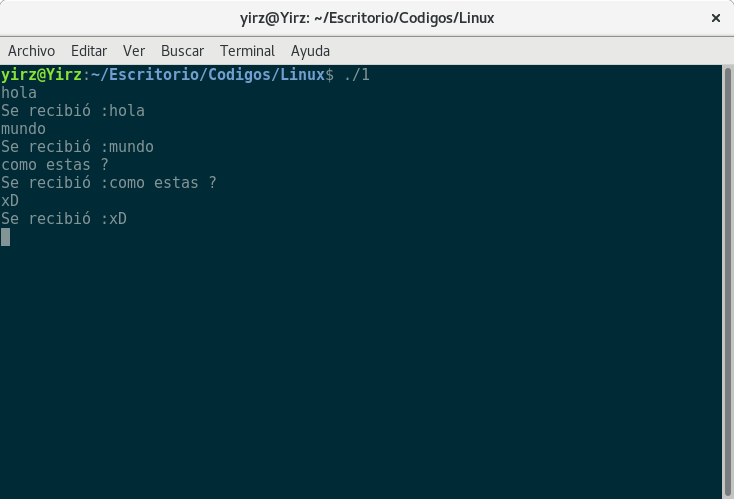
\includegraphics[scale=.3]{Imagenes/1.png}
    \end{center}
    
    \newpage
    \item Captura, compilación y ejecución del programa de creación de  hilos en Linux.
    
    \lstinputlisting{Codigos/Linux/2.c}
    \begin{center}
    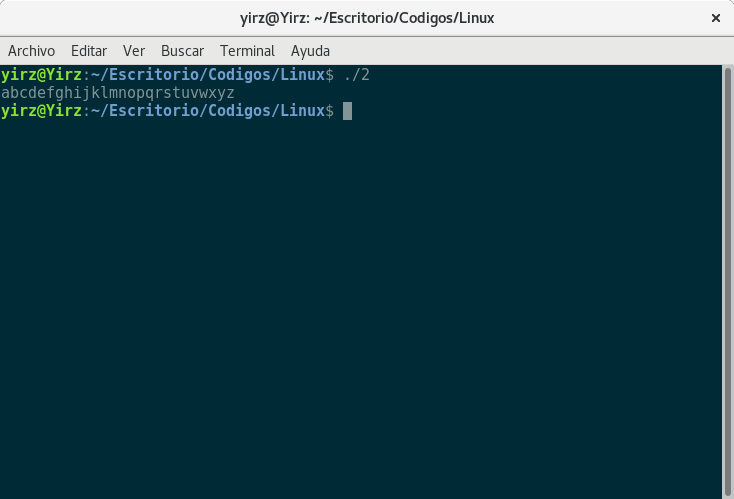
\includegraphics[scale=.3]{Imagenes/2.png}
    \end{center}
    
    \newpage
     \item Aplicación que crea un proceso hijo a partir de un proceso padre, el hijo creado a su vez creará 15 hilos. A su vez cada uno de los 15 hilos creará 10 hilos más. A su vez cada uno de los 10 hilos creará 5 hilos más. Cada uno de los hilos creados imprimirá en pantalla "Práctica No.5" si se trata de un hilo terminal o los identificadores de los hilos creados si se trata de un proceso o hilo padre. 
     
    \begin{center}
     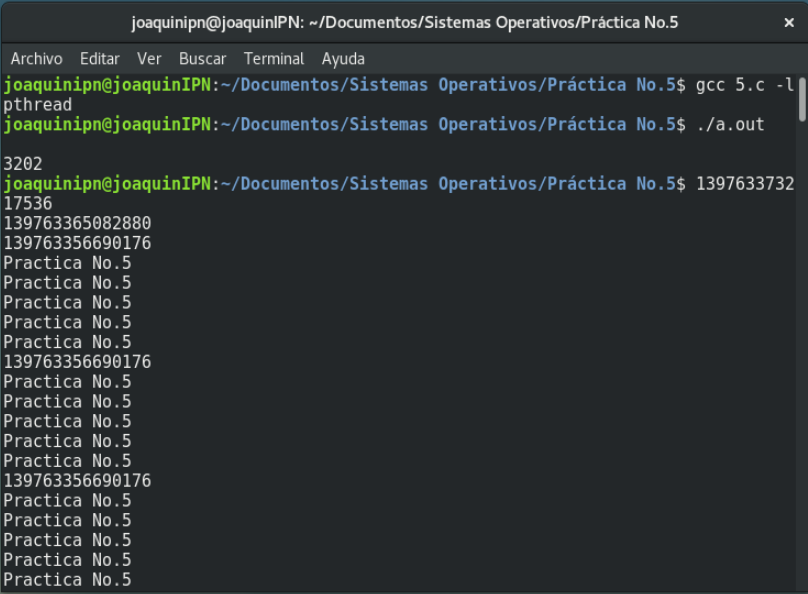
\includegraphics[scale=.3]{Imagenes/Linux/Captura de pantalla 2018-10-28 a la(s) 17.57.34.png}
     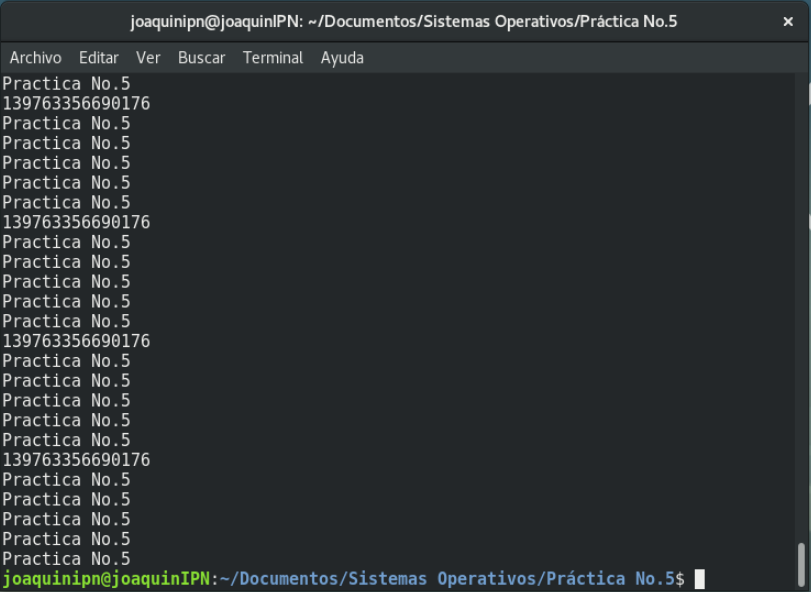
\includegraphics[scale=.3]{Imagenes/Linux/Captura de pantalla 2018-10-28 a la(s) 18.13.45.png}
      \end{center}
    
    La salida en pantalla $"Práctica No.5"$ aparece en 750 veces.
     
     \newpage
     \item  Aplicación que realiza diversas operaciones con matrices, implementanda con   hilos  en vez  de procesos. 
      \begin{center}
         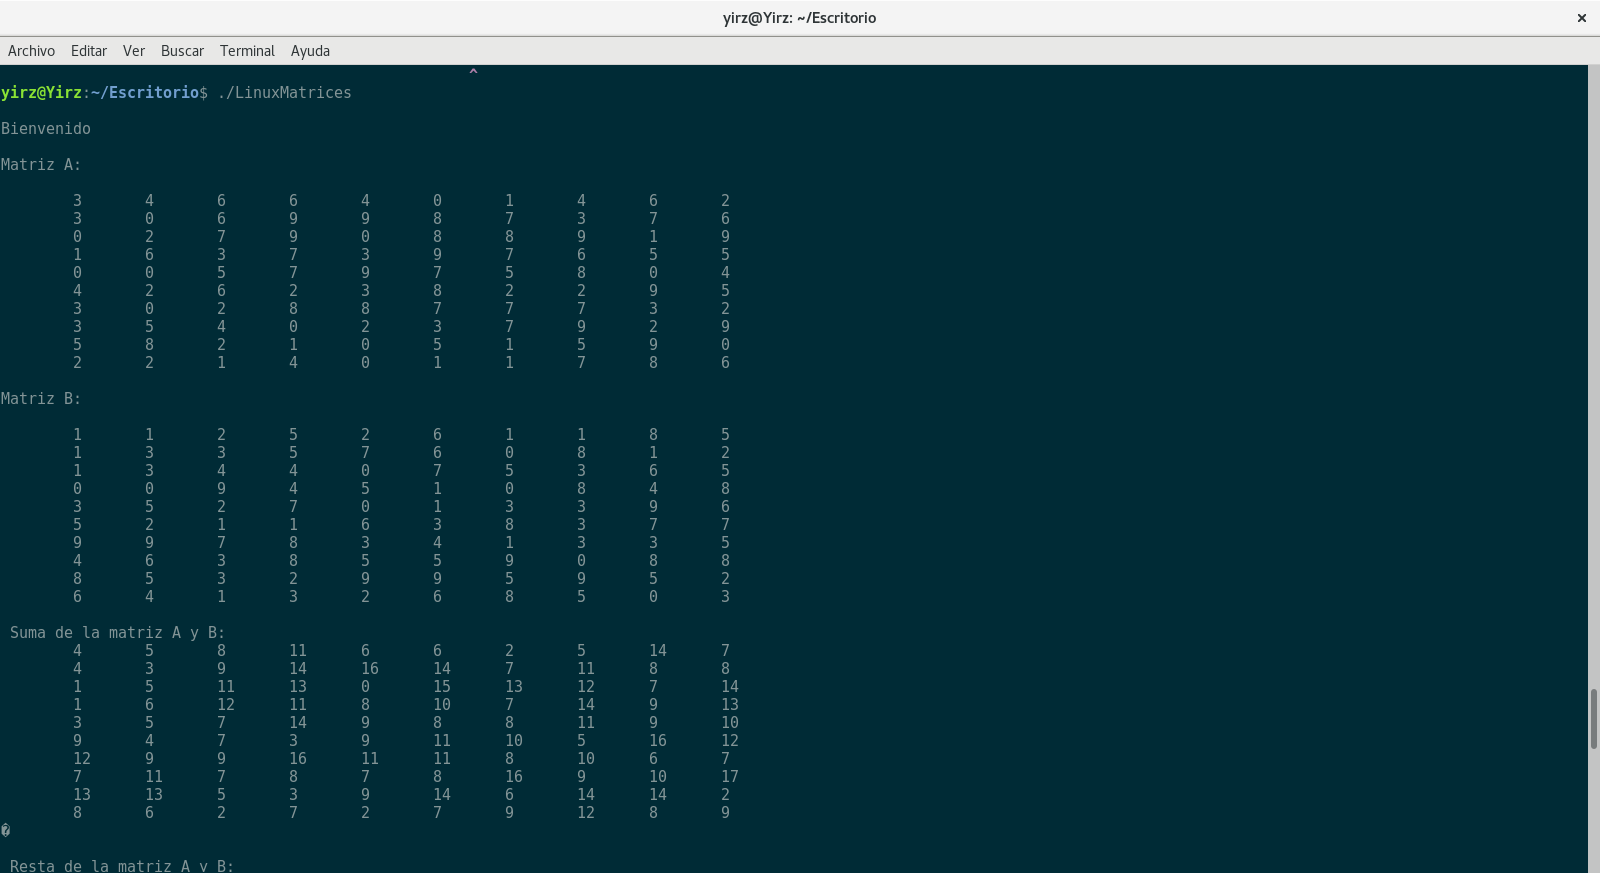
\includegraphics[scale=.25]{Imagenes/Linux/matrices1.png}\\
         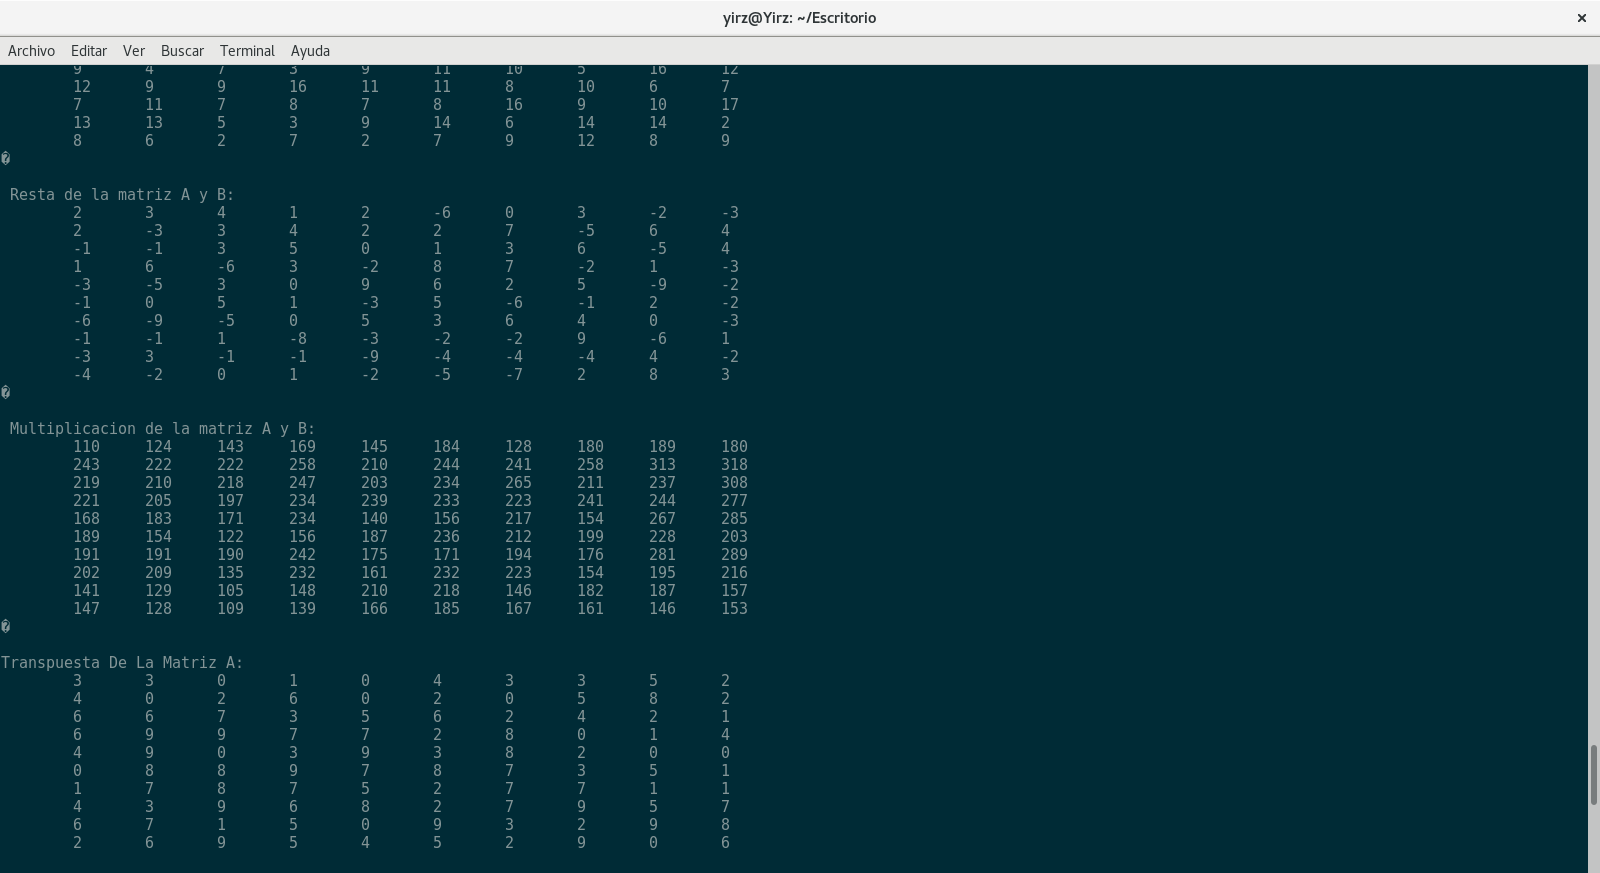
\includegraphics[scale=.25]{Imagenes/Linux/matrices2.png}\\
         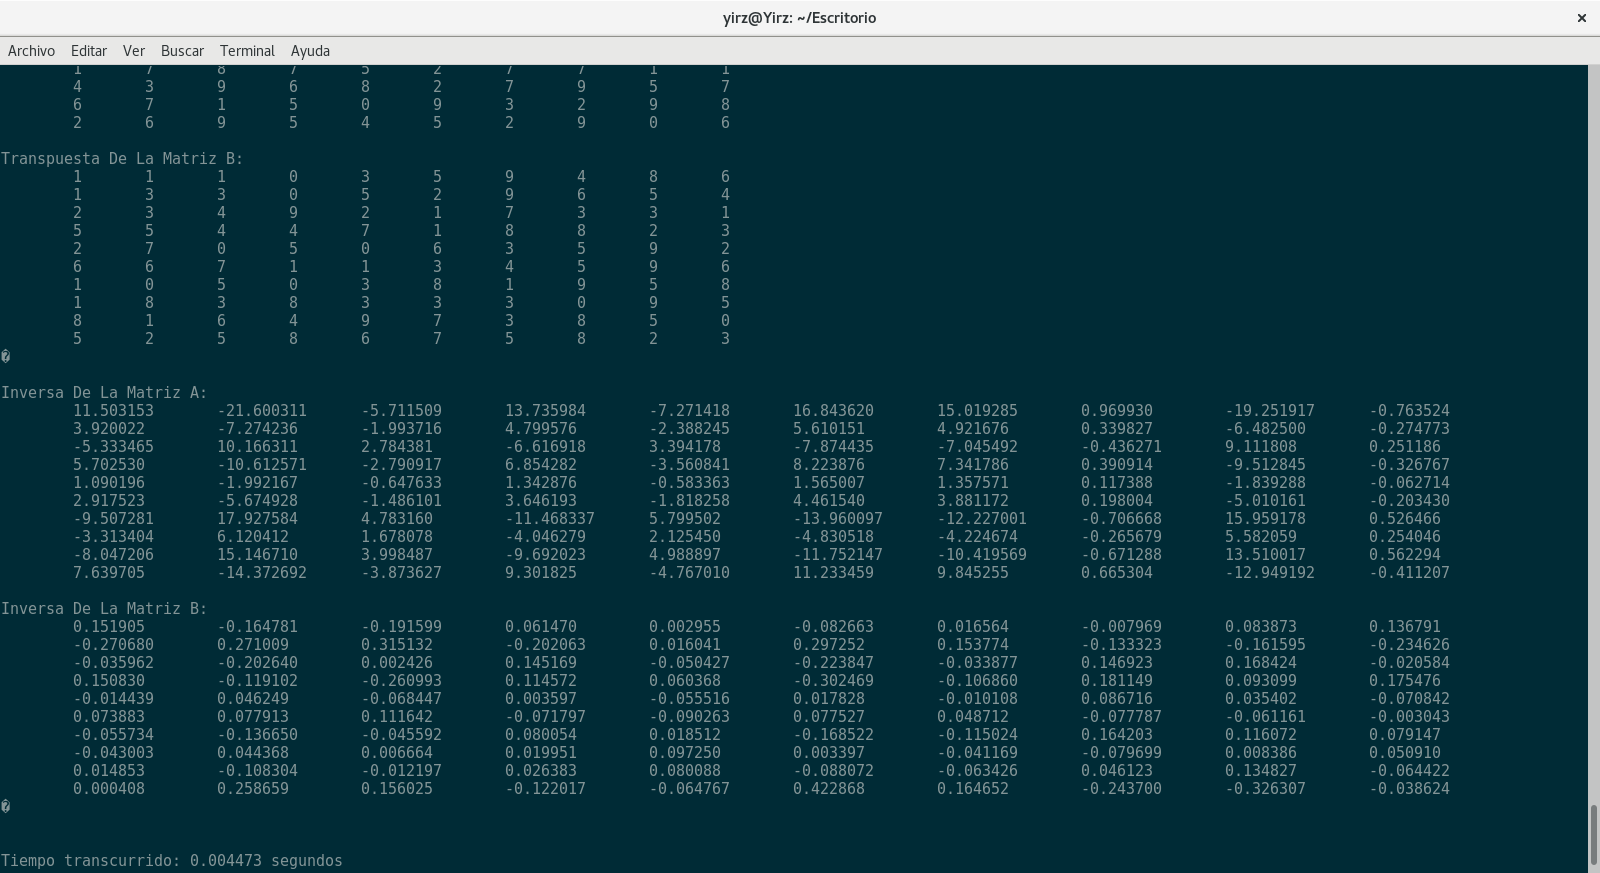
\includegraphics[scale=.25]{Imagenes/Linux/matrices3.png}
     \end{center}
     \item Aplicación  que copia los archivos y contenidos dentro una ruta específica, por cada directorio que se encuentre al momento de copiar , se deberá crear un hilo que  deberá copiar los archivos existentes en ese directorio. Nuevamente si encuentra otro directorio se creará otro hilo, así sucesivamente.Todos los hilos deben correr concurrentemente, las rutas origen y destino de copia se especifica.
    \begin{center}
         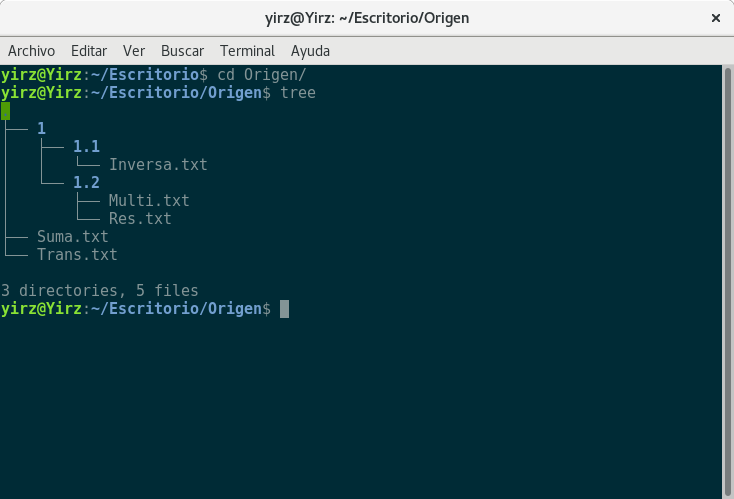
\includegraphics[scale=0.5]{Imagenes/Linux/Directorios1.png}
         
         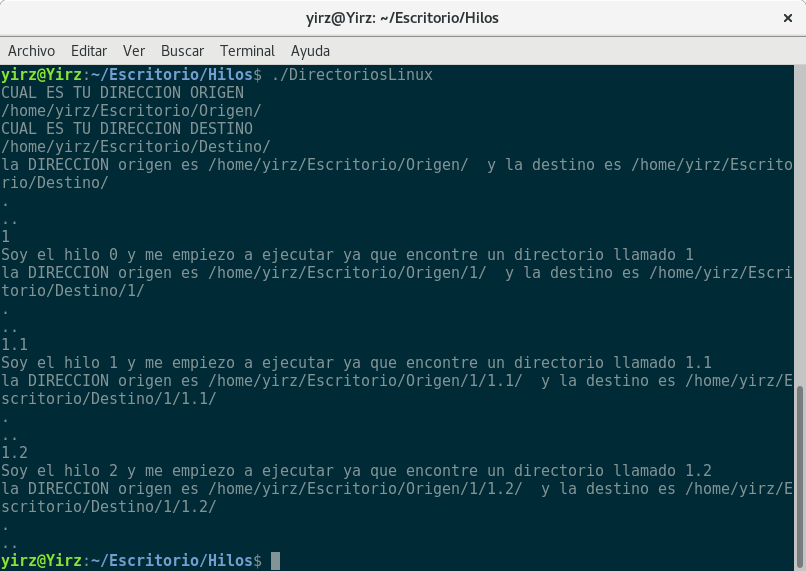
\includegraphics[scale=0.45]{Imagenes/Linux/Directorios2.png}
         
         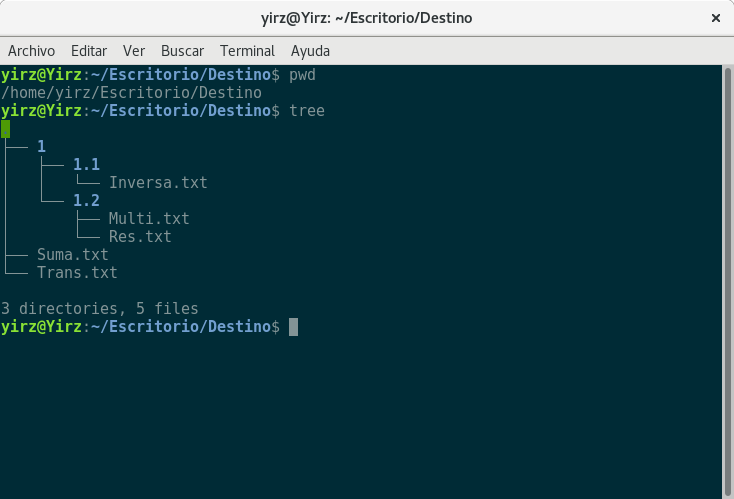
\includegraphics[scale=0.5]{Imagenes/Linux/Directorios3.png}
     \end{center}
    \end{enumerate}
    
   
    \newpage
    

\subsection{Windows}
\begin{enumerate}
    \item Capture, compile y ejecute el siguiente programa de creación de hilos en Windows.Observe su funcionamiento.
    \lstinputlisting{Codigos/Windows/Prueba.c}
    \begin{center}
        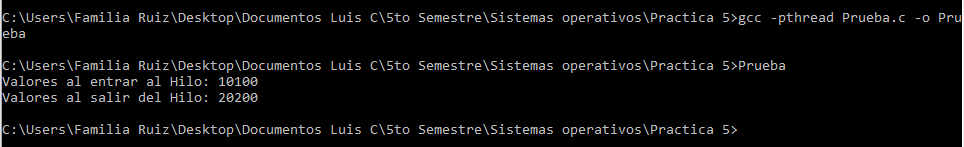
\includegraphics[scale=0.5]{Imagenes/Windows/Prueba.PNG}
    \end{center}
    \newpage
     \item Aplicación que crea un proceso hijo a partir de un proceso padre, el hijo creado a su vez creará 15 hilos. A su vez cada uno de los 15 hilos creará 10 hilos más. A su vez cada uno de los 10 hilos creará 5 hilos más. Cada uno de los hilos creados imprimirá en pantalla "Práctica No.5" si se trata de un hilo terminal o los identificadores de los hilos creados si se trata de un proceso o hilo padre. 
      \begin{center}
         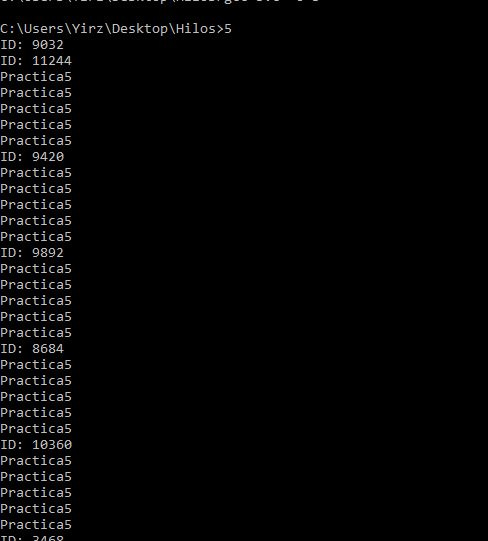
\includegraphics[scale=.5]{Imagenes/Windows/5.2.JPG}\\
         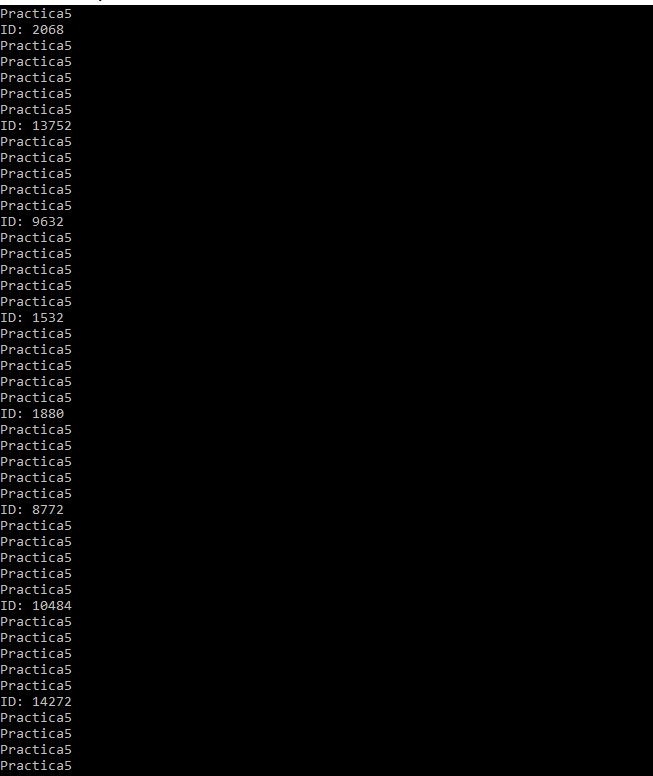
\includegraphics[scale=.40]{Imagenes/Windows/5.1.JPG}\\
     \end{center}
       La salida en pantalla $"Práctica No.5"$ aparece en 750 veces.
    \newpage     
     \item Aplicación que realiza diversas operaciones con matrices, implementanda con   hilos  en vez  de procesos. 
     \begin{center}
         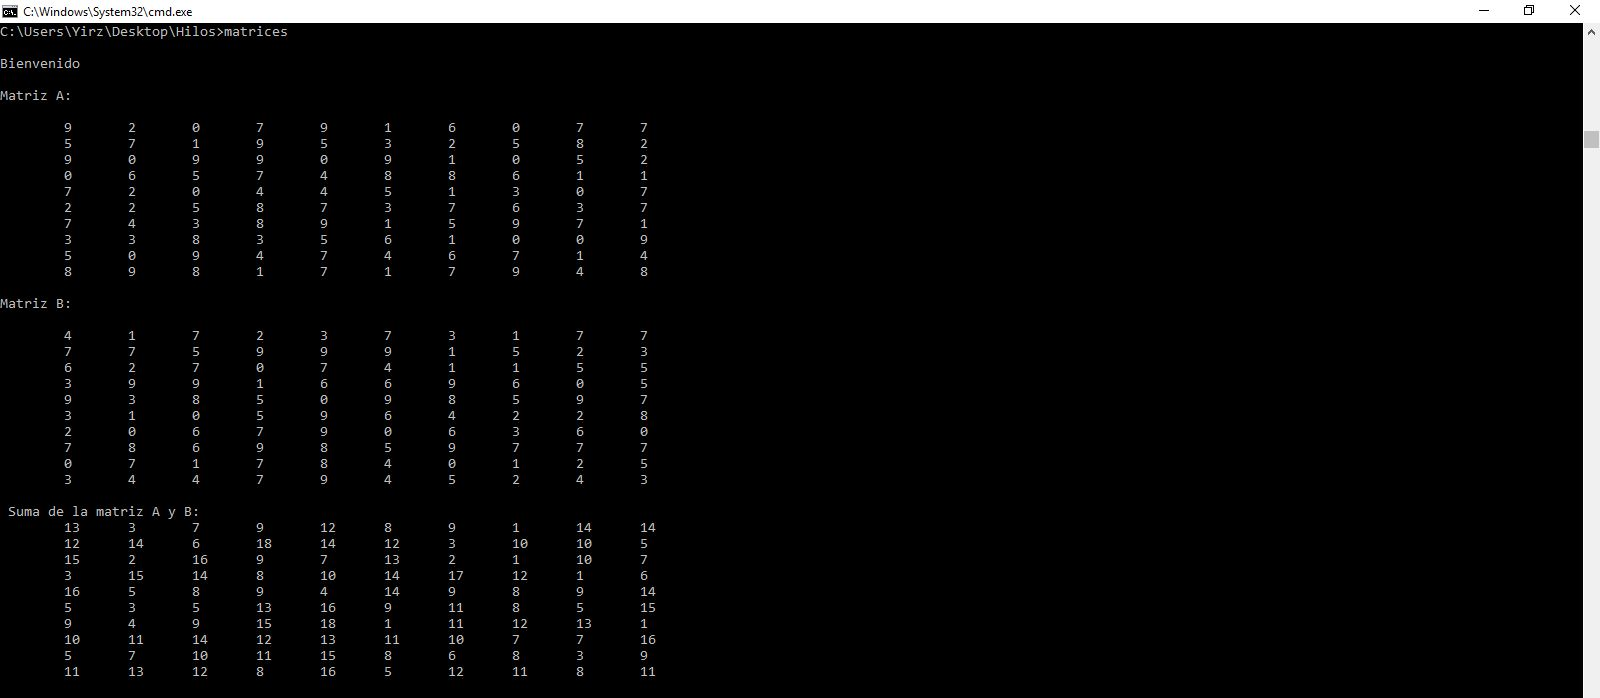
\includegraphics[scale=.3]{Imagenes/Windows/matrices1.JPG}\\
         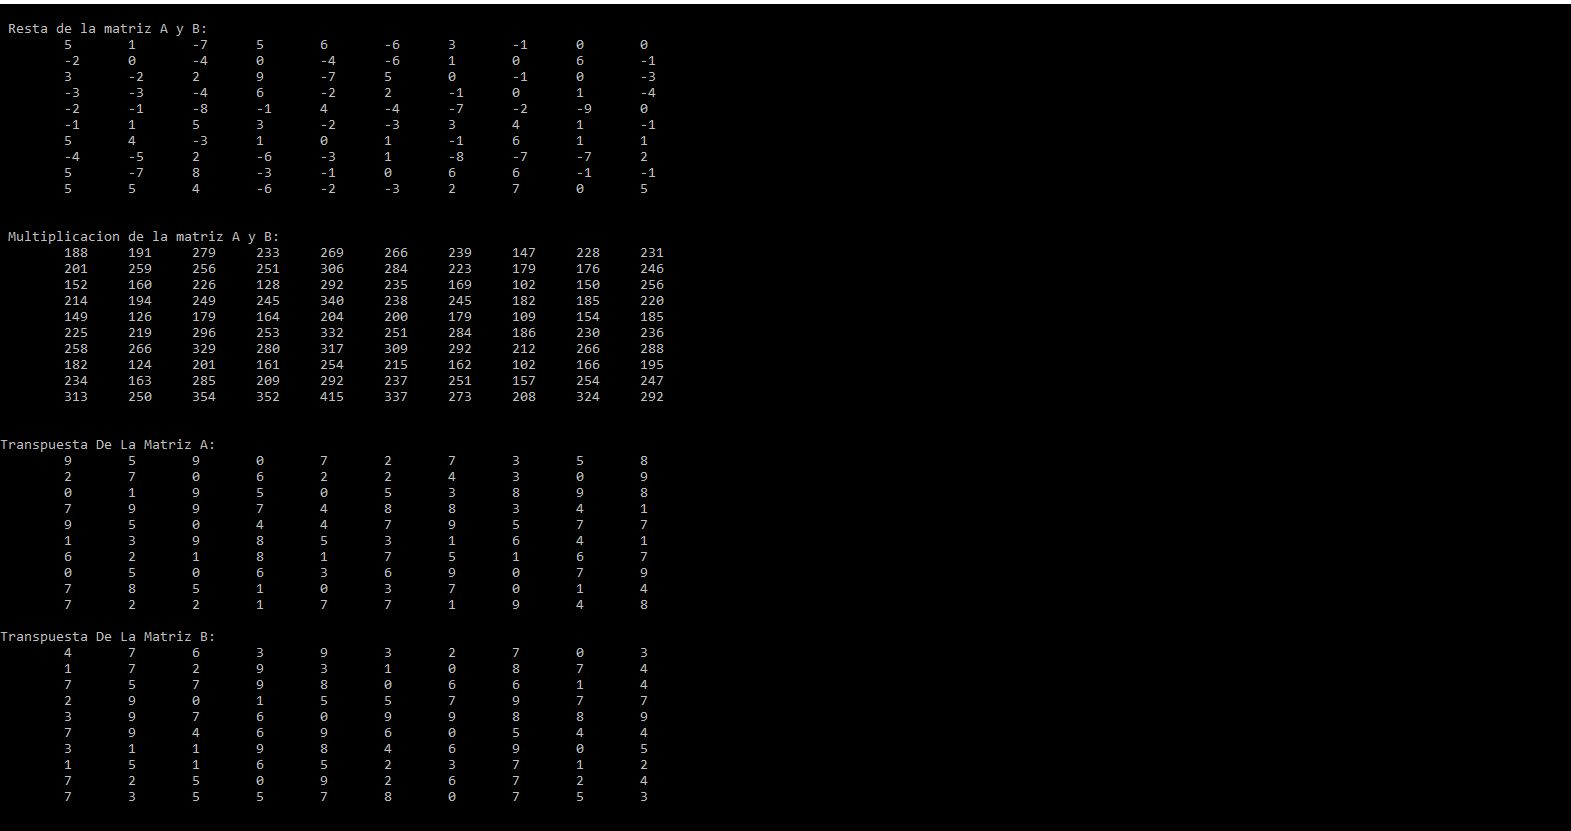
\includegraphics[scale=.3]{Imagenes/Windows/matrices2.JPG}\\
         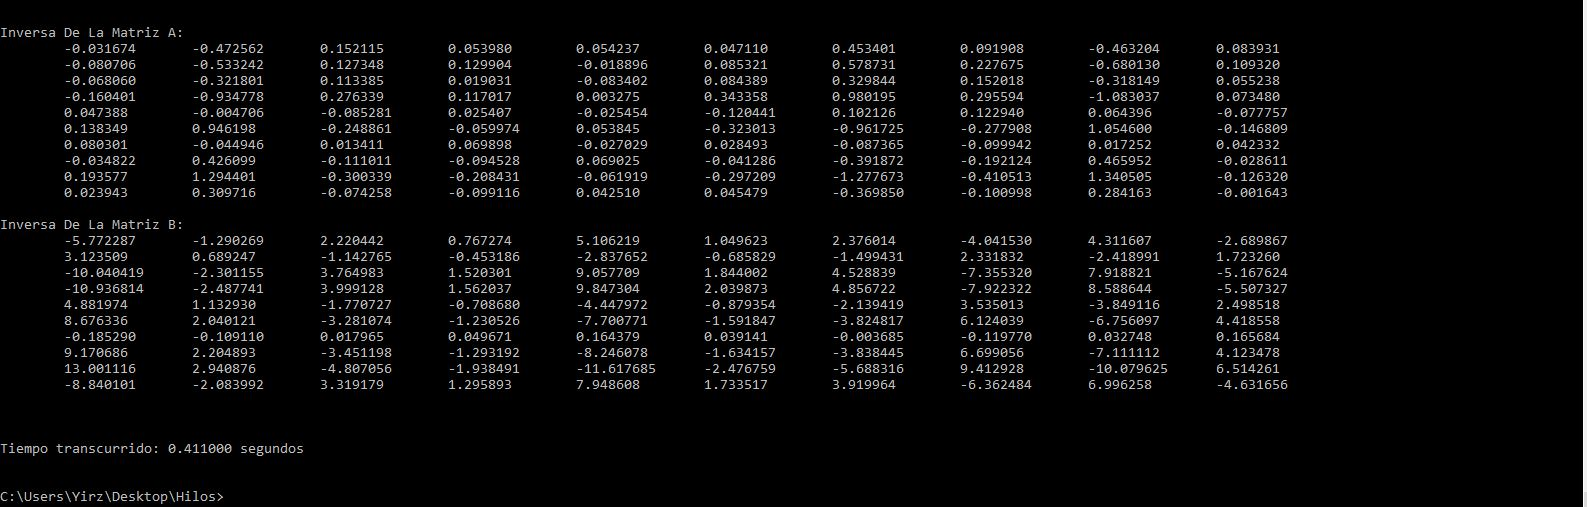
\includegraphics[scale=.3]{Imagenes/Windows/matrices3.JPG}
     \end{center}
     \item Aplicación  que copia los archivos y contenidos dentro una ruta específica, por cada directorio que se encuentre al momento de copiar , se deberá crear un hilo que  deberá copiar los archivos existentes en ese directorio. Nuevamente si encuentra otro directorio se creará otro hilo, así sucesivamente.Todos los hilos deben correr concurrentemente, las rutas origen y destino de copia se especifica.
     \begin{center}
         
\includegraphics[scale=0.80]{Imagenes/Windows/Driectorio1.jpg}\\
         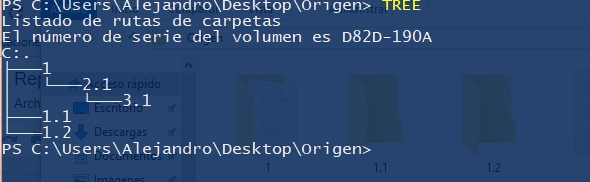
\includegraphics[scale=0.75]{Imagenes/Windows/Driectorio2.jpg}\\
         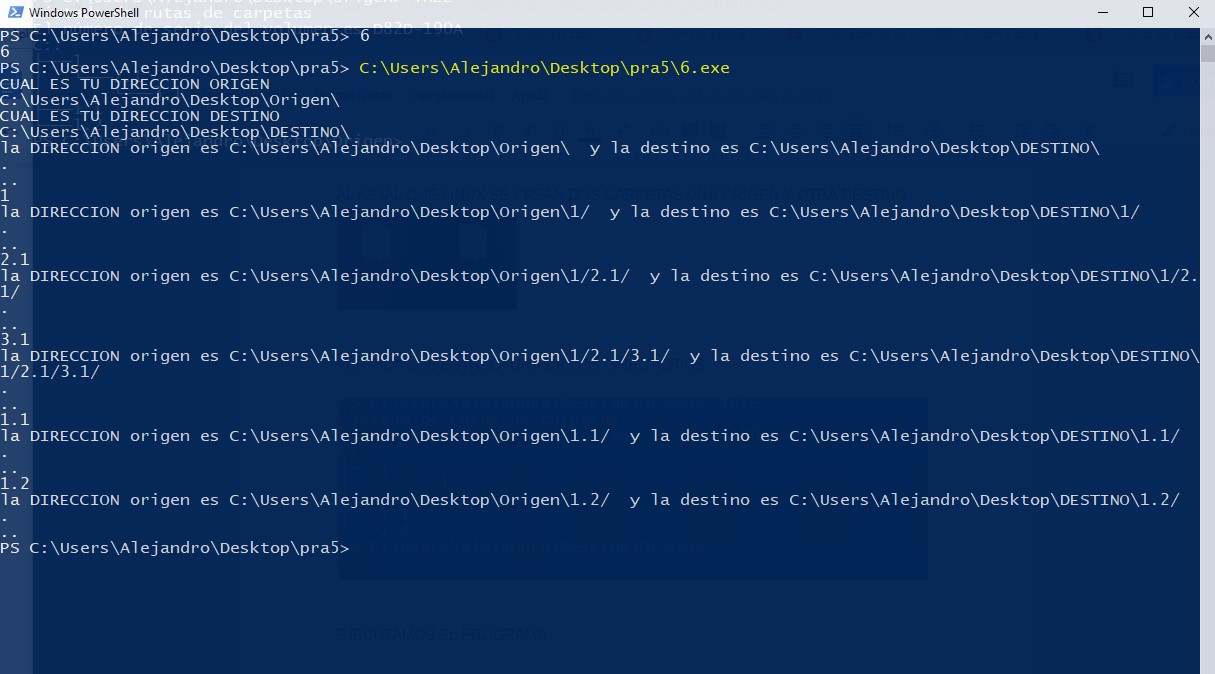
\includegraphics[scale=0.5]{Imagenes/Windows/Driectorio3.jpg}\\
         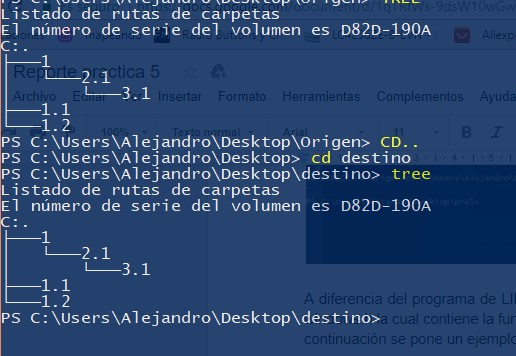
\includegraphics[scale=0.75]{Imagenes/Windows/Driectorio4.jpg}
     \end{center}
\end{enumerate}
    
\newpage
\subsection{Código Fuente.}
   \subsubsection{Linux}
   
    \begin{itemize}
       \item \textbf{Árbol de hilos}
         \lstinputlisting{Codigos/Linux/5.c}
        \item \textbf{Operaciones con Matrices}
        \lstinputlisting{Codigos/Linux/LinuxMatrices.c}
        \item \textbf{Directorios}
         \lstinputlisting{Codigos/Linux/DirectoriosLinux.c}
   \end{itemize}
        
   \subsubsection{Windows}
   \begin{itemize}
       \item \textbf{Árbol de hilos}
       \lstinputlisting{Codigos/Windows/5.c}
        \item \textbf{Operaciones con Matrices}
         \lstinputlisting{Codigos/Windows/matrices.c}
        \item \textbf{Directorios}
        \lstinputlisting{Codigos/Windows/DirectoriosWindows.c}
   \end{itemize}

\section{Observaciones.}

Se tienen las siguientes obervaciones: 
 \begin{itemize}
    \item Se observa que los hilos, a diferencia de los procesos comparten recursos. La compartición de la memoria permite a los hilos  comunicarse sin usar ningún mecanismo de comunicación inter-proceso del sistema operativo como fue en las aplicaciones de contrucción de un árbol de hilos y en la l aplicación, que copia los archivos y contenidos dentro una ruta específica.
    \item La conmutación de contexto es más rápida gracias al extenso compartir de recursos
    \item No hay protección entre las hilos. Un hilo puede escribir en la pila de otra hilo del mismo proceso.
 
 \end{itemize}


\section{Análisis Crítico.}
En cuanto a velocidades  se pude analizar, que la versión programación concurrente tiene la capacidad de ser mas rápido al momento de la ejecución que en la programación secuencial, por ejemplo en el programa concurrente de operaciones con matrices el tiempo de ejecución fue de 2022 milisegundos mientras que en la versión secuencial fue de 0.006783 segundos, el tiempo de ejecución concurrete de creación de procesos por sustitución de código fue de 0.000218 segundos, por lo tanto la ejecución más rápida fue por creación de procesos por copia exacta de código. Sin embargo , cuando se asocia una proceso ligeron la velocidad fue de  0.004473 segundos. 

La version concurrente tiene la capacidad de ser mas rapido al momento de la ejecucion. Se debe toman en cuenta el estado actual de las variables a manejar con la programacion multihilo pues de perder la nocion de estas puede ocasionar resultados no deseado, aúmentado el tiempo de ejecución.


\newpage
\section{Conclusiones.}

Finalmente, por medio de la presente práctica se pudo corrobarar las diferencias entre procesos y porcesos ligeros (hilos),como sabemos un proceso es una entidad relativamente independiente que dispone de su propio espacio de direcciones, su propia información de estado y que utiliza los mecanismos de comunicación entre procesos que le proporciona el sistema operativo para comunicarse con otros procesos. Por otro lado, un hilo es una entidad más reducida capaz de convivir junto a otros hilos bajo el contexto de un único proceso, permitiendo compartir la información de estado, el área de memoria y/o los recursos asociados a ese proceso.


Dentro de un proceso puede haber uno o más hilos de control cada uno con:

\begin{itemize}
       \item Un estado de ejecución (en ejecución, listo, bloqueado)
        \item Un contexto de procesador, que se salva cuando no esté ejecutándose.
        \item Una pila de ejecución.
        \item Algún almacenamiento estático para variables locales.
        \item Acceso a la memoria y a los recursos de ese trabajo que comparte con los otros hilos.
   \end{itemize}
Por ende, los beneficios clave de los hilos se derivan de las implicaciones del rendimiento: se tarda menos tiempo en crear un nuevo hilo de un proceso que ya existe, en terminarlo, y en hacer un cambio de contexto entre hilos de un mismo proceso. Al someter a un mismo proceso a varios flujos de ejecución se mantiene una única copia en memoria del código, y no varias.

\end{document}